\chapter{Object Detection State-of-Art}
\label{chapter:object_detection}

This chapter studies the current CNN-based state-of-art object detectors, alongside the benchmarks and metrics used for their evaluation. Based on this study, one object detector is chosen and described.\\

\vspace{-0.4cm}
The task of a general-purpose object detector is to locate and classify existing objects in an image from predefined categories. The most common way to label and output the coordinates of the located object is to draw a bounding box around it, as represented in Fig.~\ref{fig:bounding_box}. State-of-art object detectors are DNN-based and their backbone network for feature extraction consists (or is inspired) in the networks for image classification mentioned in the section \ref{section:popular_models}, excluding the last fully connected layers~\cite{jiao:obj_survey}.   

\begin{figure}[!htb]
  \centering
  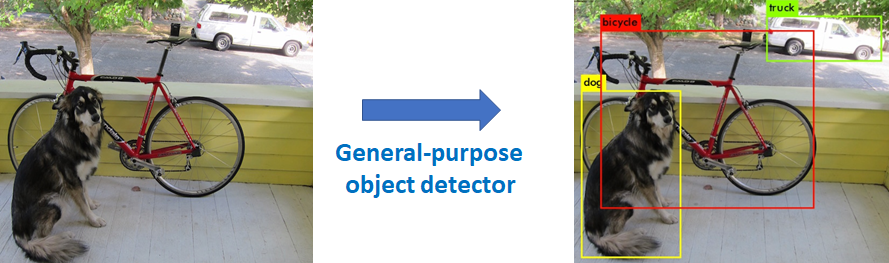
\includegraphics[width=0.7\textwidth]{Figures/bounding_box.png}
  \caption{Example of bounding box usage to locate objects in an image (adapted from~\cite{Redmon2015YouOL}).}
  \label{fig:bounding_box}
\end{figure}
\vspace{-0.2cm}

\section{Benchmarks and metrics}
\label{section:benchmarks}

Two of the most common benchmarks for general-purpose object detection are PASCAL VOC 2007/2012 and Microsoft COCO~\cite{zhao:obj_survey}. The official metric for measuring the performance of detectors is based on the mean average precision (mAP) with small variations between both benchmarks. This metric compares the predicted bounding boxes and labels with the ground truth data, which provides the true labels of each object in an image including the class and the coordinates of the true bounding box.   

Object detection is simultaneously a regression (object bounding box) and a
classification (object class) task. The process for calculating the mAP metric
is summed up in Fig.~\ref{fig:map}. Usually, the model outputs more boxes than
actual objects, which indicates the presence of boxes with low
confidence. Therefore, the first step is to label the predicted bounding boxes
as true or false detections with respect to the ground truth bounding boxes. The
Intersection over Union (IoU) is an evaluation metric that measures the accuracy
of the localization task by calculating the ratio of the area of overlap and the
area of union between the predicted and the ground truth bounding boxes. The
predicted bounding box is considered a true detection if its IoU score is above
a given IoU threshold, otherwise, it is a false detection. Duplicated bounding
boxes and wrong classifications are also false detections.

The average precision (AP) of each class is calculated based on the precision and recall metrics. The precision measures the ratio of the true detections and the total number of objects detected~\cite{unlu:real_app}. The recall measures the ratio of the true detections and the total number of objects in the dataset~\cite{unlu:real_app}. A high precision indicates that it is likely that a true detection is, in fact, a correct detection while a high recall means that the detector will positively detect all objects in the dataset.

Each bounding box has a score associated which indicates how likely that box contains an object. To calculate the AP of each class, the precision-recall curve is computed from the detections of the model by varying the score threshold. The AP corresponds to the area under that curve and is typically computed by numerical integration. After the AP of all classes is calculated, the mAP is determined as the average of all the APs, resulting in a value between 0 and 100\%. Therefore, the mAP metric allows to evaluate both classification and localization and is designed to penalize the algorithms for missing object instances, for duplicate detections of one instance, for false positive detections and for specializing in some classes, resulting in worse performances in other classes~\cite{jiao:obj_survey}.

\begin{figure}[!htb]
  \centering
  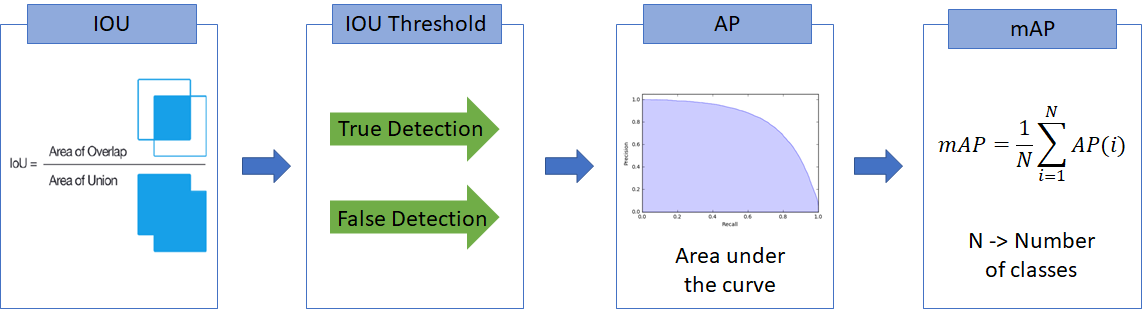
\includegraphics[width=0.9\textwidth]{Figures/mAP.png}
  \caption{Steps for obtaining the mean average precision (adapted from~\cite{unlu:real_app}).}
  \label{fig:map}
\end{figure}

The PASCAL VOC datasets contain 20 object categories (e.g., person, bicycle, dog) spread over 11k images, from which over 27k object instances are labeled with bounding boxes~\cite{jiao:obj_survey}. This benchmark considers only one IoU threshold of 0.5 to obtain the mAP. On the other hand, the COCO dataset is composed by 300k images with an average of 7 object instances per image from a total of 80 categories~\cite{zhao:obj_survey}. This benchmark considers ten IoU thresholds (from 0.5 to 0.95 with an interval of 0.05) and the mAP is obtained by averaging the mAPs calculated for each IoU threshold. Considering several IoU thresholds tends to reward models that are better at precise localization and penalizes the algorithms with a high number of bounding boxes with wrong classifications.

\vspace{-0.4cm}
\section{Comparison between object detectors}
\label{section:obj_det_comp}
\vspace{-0.1cm}

Several studies have been conducted for comparing the performance of the state-of-art object detectors~\citep{{jiao:obj_survey, liu:obj_survey, zhao:obj_survey}}. Object detectors can be divided into two categories: two-stage detectors (region proposal based) and one-stage detector (regression/classification based).

Two-stage detectors follow the traditional object detection pipeline by firstly scanning the whole scenario and then focusing on regions of interest. Thus, the first stage consists in generating region proposals (i.e., candidate bounding boxes). In the second stage, features are extracted from each candidate box in order to perform the classification and bounding box regression tasks. The most popular two-stage detectors are R-CNN, Fast R-CNN, Faster R-CNN, Mask R-CNN and R-FCN~\citep{{jiao:obj_survey, zhao:obj_survey, feng:obj_survey}}.

One-stage detectors treat object detection as a regression/classification problem by adopting a unified framework to obtain the labels and locations directly. These detectors map straightly from image pixels to bounding box coordinates and class probabilities by proposing predicted boxes directly from input images without the region proposal step. The most common one-stage detectors are Yolo and its successors Yolov2 and Yolov3, SSD and its successor DSSD and RetinaNet~\citep{{jiao:obj_survey, zhao:obj_survey, feng:obj_survey}}. 

The selection between one-stage and two-stage detectors resides on a choice between speed and accuracy. Two-stage detectors present higher localization and object recognition accuracy while one-stage detectors achieve higher inference speed. Table~\ref{tab:obj_det_comp} summarizes the mAP metric for both PASCAL VOC 2007 and COCO datasets and the inference time of each of the above-mentioned object detectors. For the COCO dataset, besides the official mAP metric (i.e., obtained from ten IoU thresholds), the mAP with only one IoU of 0.5 is also shown. 

\begin{table}[!htb]
    \footnotesize
    \centering
    \caption{Comparison of the performance of several object detectors.}
    \label{tab:obj_det_comp}
    \begin{tabular}{|c|c|c|c c|c c|c|c|}
    \hline
    
    \multirow{2}{*}{Type} & \multirow{2}{*}{Detector} & PASCAL VOC07 & \multicolumn{2}{|c|}{COCO} & \multicolumn{2}{|c|}{Inference time} & \multirow{2}{*}{Backbone} & \multirow{2}{*}{Hardware} \\ \cline{3-7}
    & & $mAP$ & $mAP$ & $mAP_{50}$ & ms & fps & & \\ \hline
    {\multirow{5}{*}{\rotatebox[origin=c]{90}{Two-stage}}} & R-CNN~\cite{feng:obj_survey} & 66 & --- & --- & 10000 & 0.1 & AlexNet & \multirow{16}{*}{Titax X GPU} \\ \cline{2-8}
    & Fast R-CNN~\cite{{jiao:obj_survey, feng:obj_survey}} & 70 & 19.7 & 35.9 & 2000 & 0.5 & VGG16 & \\ \cline{2-8}
    & Faster R-CNN~\cite{{jiao:obj_survey, feng:obj_survey}} & 73.2 & 21.9 & 42.7 & 167 & 6 & VGG16 & \\ \cline{2-8}
    & R-FCN~\cite{{jiao:obj_survey, zhao:obj_survey}} & \cellcolor{gray!25}83.6 & 29.9 & 51.9 & 170 & 5.9 & ResNet-101 & \\ \cline{2-8}
    & Mask R-CNN~\cite{{jiao:obj_survey, feng:obj_survey}} & --- & \cellcolor{gray!25}39.8 & \cellcolor{gray!25}62.3 & 303 & 3.3 & ResNeXt-101 & \\ \cline{1-8}
    
    {\multirow{13}{*}{\rotatebox[origin=c]{90}{One-stage}}} & YOLO~\cite{feng:obj_survey}  & 63.4 & --- & --- & \cellcolor{gray!25}22 & \cellcolor{gray!25}45 & GoogLeNet & \\ \cline{2-8}
    & YOLOv2-544~\cite{{jiao:obj_survey, zhao:obj_survey}} & 73.4 & 21.6 & 44 & \cellcolor{gray!25}25 & \cellcolor{gray!25}40 & DarkNet-19 & \\ \cline{2-8}
    & SSD-300~\citep{{jiao:obj_survey, zhao:obj_survey}} & 74.3 & 23.2 & 41.2 & \cellcolor{gray!25}21.7 & \cellcolor{gray!25}46 & \multirow{2}{*}{VGG-16} & \\ \cline{2-7}
    & SSD-512~\citep{{jiao:obj_survey, zhao:obj_survey}} & 76.8 & 26.8 & 46.5 & 52.6 & 19 & & \\ \cline{2-8}
    & SSD-321~\citep{{jiao:obj_survey, Redmon2018YOLOv3AI}} & --- & 28 & 45.4 & 61 & 16.4 & \multirow{4}{*}{ResNet-101} & \\ \cline{2-7}
    & SSD-513~\citep{{jiao:obj_survey, feng:obj_survey, Redmon2018YOLOv3AI}} & 76.8 & 31.2 & 50.4 & 125 & 8 & & \\ \cline{2-7}
    & DSSD-321~\citep{{jiao:obj_survey, zhao:obj_survey, Redmon2018YOLOv3AI}} & 78.6 & 28 & 46.1 & 85 & 11.8 & & \\ \cline{2-7}
    & DSSD-513~\citep{{jiao:obj_survey, Redmon2018YOLOv3AI}} & --- & 33.2 & 53.3 & 156 & 6.4 & & \\ \cline{2-8}
    & YOLOv3-320~\cite{Redmon2018YOLOv3AI} & --- & 28.3 & 51.5 & \cellcolor{gray!25}22 & \cellcolor{gray!25}45.5 & \multirow{3}{*}{DarkNet-53} & \\ \cline{2-7}
    & YOLOv3-416~\cite{Redmon2018YOLOv3AI} & --- & 31 & 55.3 & \cellcolor{gray!25}29 & \cellcolor{gray!25}34.5 & & \\ \cline{2-7}
    & YOLOv3-608~\cite{Redmon2018YOLOv3AI} & --- & 33 & 57.9 & 51 & 19.6 & & \\ \cline{2-9}
    & RetinaNet-500~\citep{jiao:obj_survey, Redmon2018YOLOv3AI} & --- & 34.4 & 53.1 & 90 & 11.1 & \multirow{2}{*}{ResNet-101} & \multirow{2}{*}{M40 GPU} \\ \cline{2-7}
    & RetinaNet-800~\citep{jiao:obj_survey, Redmon2018YOLOv3AI} & --- & 37.8 & 57.5 & 198 & 5 & & \\ \hline
    
    \end{tabular}
\end{table}
\vspace{-0.2cm}

The best performance for both PASCAL VOC and COCO datasets are achieved by two-stage detectors, namely R-FCN and Mask R-CNN. Higher frame rates are achievable with one-stage detectors such as YOLO (and its successors) and one version of the SSD detector. There are several versions available for the same detectors which mainly differ in the size of the input feature maps of the first layer. However, the topology of the network is the same for any version. For instance, YOLOv3 has three versions with input feature maps of  320x320, 416x416 or 608x608. Bigger input feature maps tend to lead to higher accuracy but lower speed. In the case of the SSD detector, some versions use VGG-16 which results in accelerated performance and others use ResNet-101 for higher accuracy. 

Within these detectors, YOLOv3 is the one that presents the best trade-off between accuracy and execution time (for the 320 and 416 versions). Therefore, this is the object detector that will be implemented in the scope of this work. 

\section{YOLOv3 detector}
\label{section:yolo}

Fig.~\ref{fig:yolov3} exemplifies the process flow of the YOLOv3 detector for an input feature map of 416x416. The input image is resized at the beginning of the process as the detector allows different input resolutions. The YOLOv3 network block is responsible for extracting features using the Darknet-53 backbone and for returning candidate bounding boxes from those features for three different scales (52x52, 26x26 and 13x13). Candidate bounding boxes are then filtered based on their objectness score and the score of each class. Finally, non-maximum suppression is used to remove multiple detections of the same object.  

\begin{figure}[!htb]
  \centering
  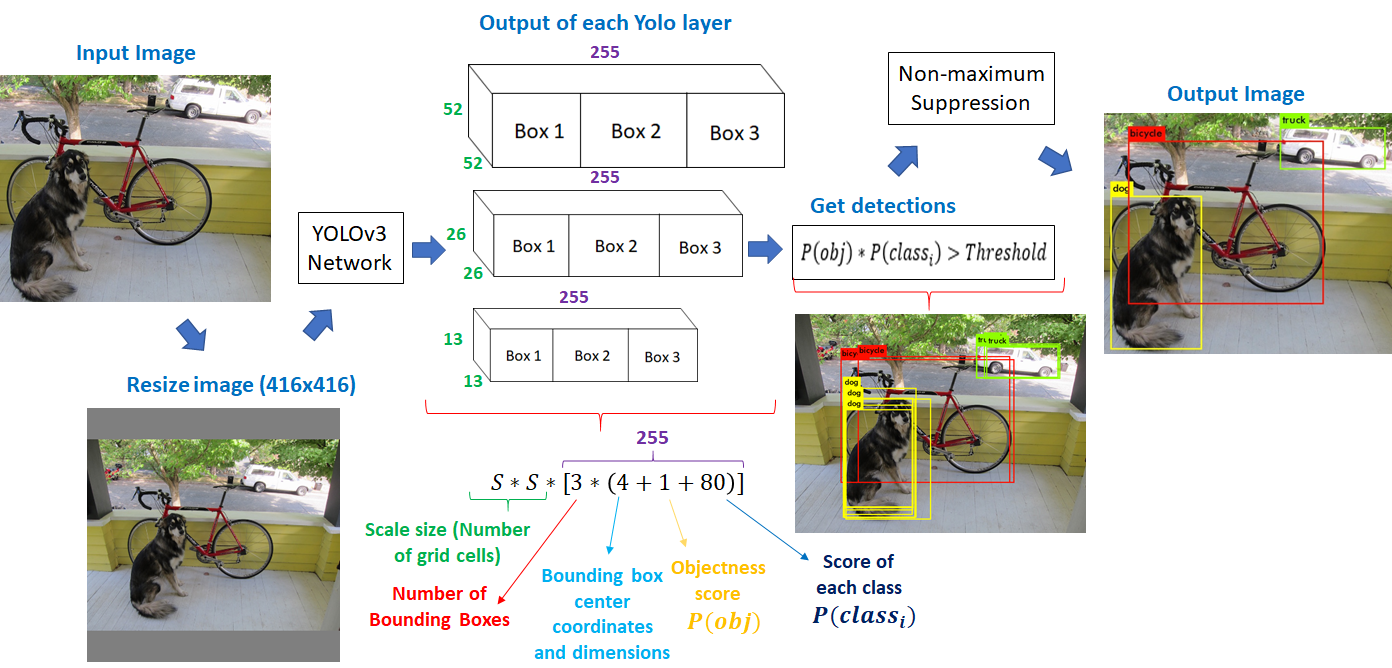
\includegraphics[width=\textwidth]{Figures/yolov3.png}
  \caption{YOLOv3 process flow.}
  \label{fig:yolov3}
\end{figure}

\subsection{YOLOv3 network}

The CNN-based YOLOv3 network is represented in Fig.~\ref{fig:yolov3_ntw}. This network is composed by 75 convolutional layers, 23 shortcut layers, 3 yolo layers, 2 upsample layers and 4 route layers, making a total of 107 layers. The two route layers after the yolo layers only copy the output of a former layer without concatenating with the output of the previous layer. All convolutional layers include batch-normalization and use Leaky ReLU (with $a$ = 0.1) as activation function, except from the convolutional layer exactly before of each yolo layer, which does not include batch-normalization and uses a linear activation function. There are no fully connected layers and convolutional layers with stride 2 are used instead of maxpool layers. One can also observe that every time the feature map is downsampled by a factor of four, the depth (i.e., number of channels) is duplicated. 3x3 convolutions are done with zero-padding in order to keep the same size between input and output feature maps.

\begin{figure}[!htb]
  \centering
  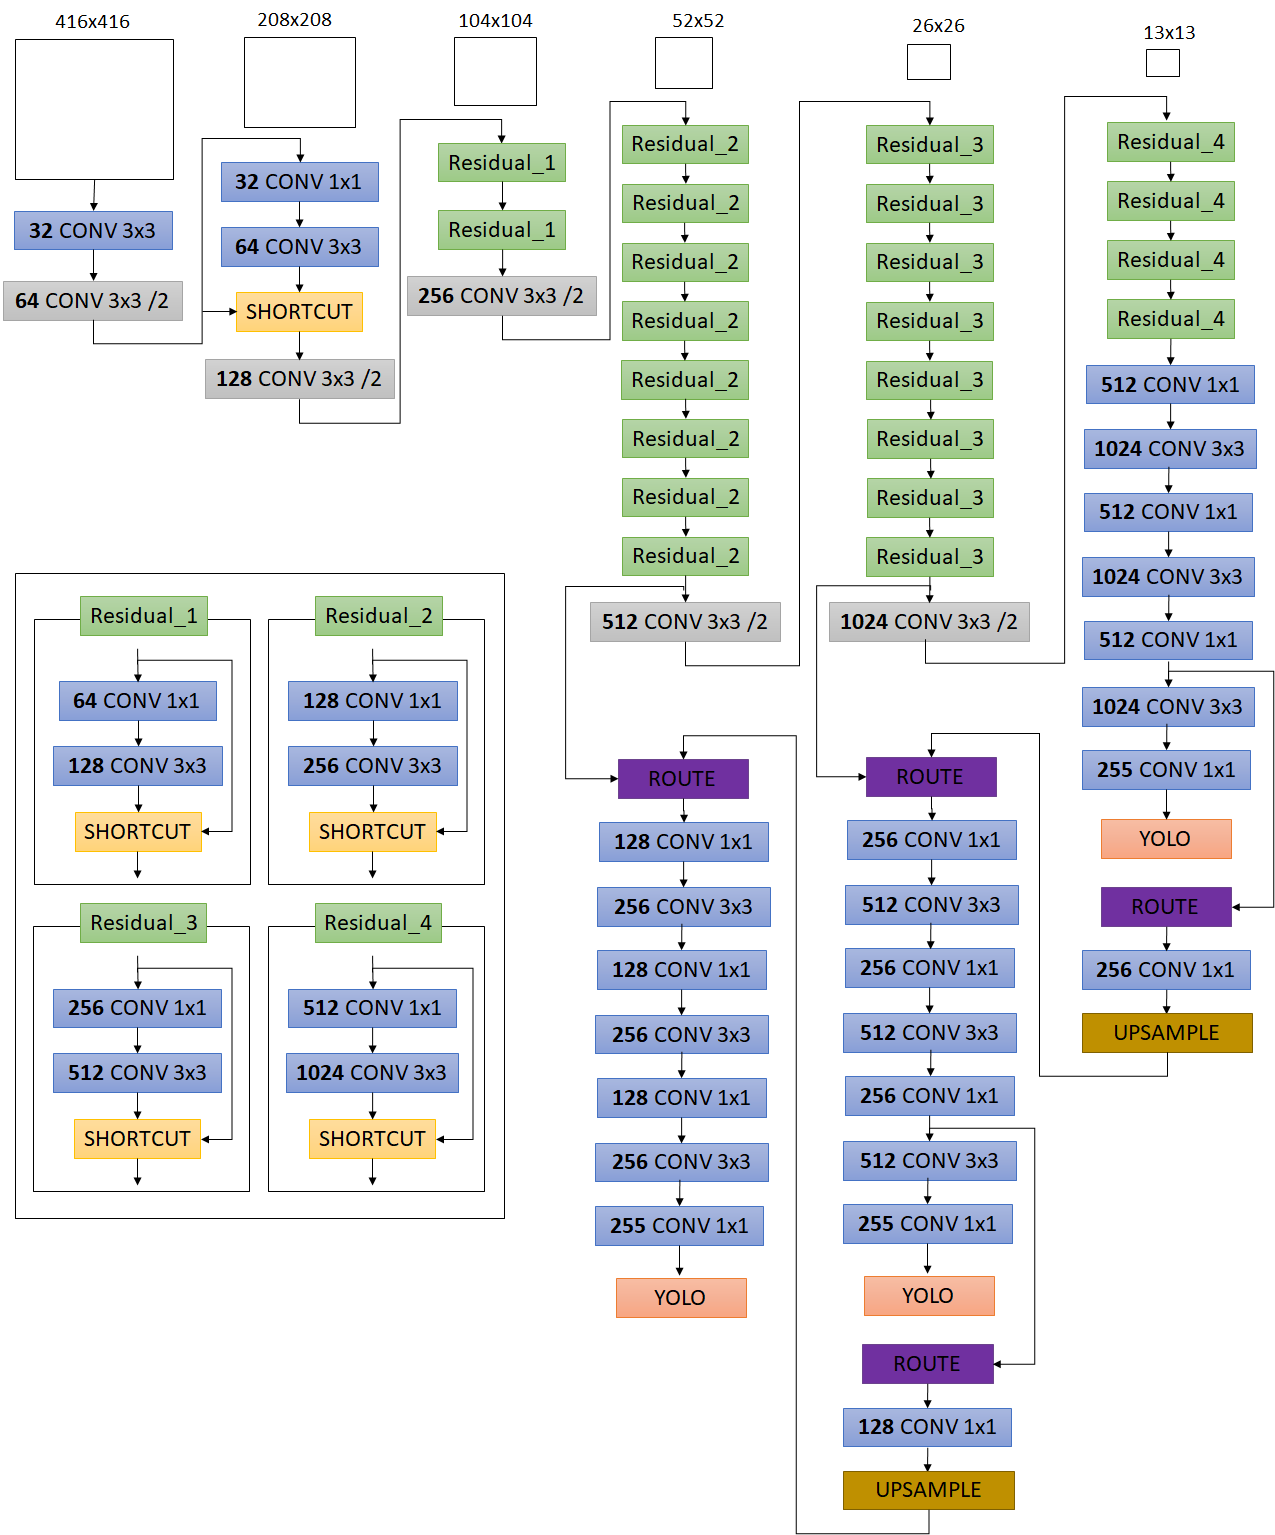
\includegraphics[width=0.9\textwidth]{Figures/yolov3_ntw.png}
  \caption{YOLOv3 Network.}
  \label{fig:yolov3_ntw}
\end{figure}

This network is inspired on some concepts from popular DNN models. For instance, the kernels are mostly 3x3 and 1x1 to reduce the number of weights as first introduced by GoogLeNet. A ResNet-alike structure is followed through the shortcut layers, thereby enhancing feature learning in deep networks. As the network goes deeper, due to downsampling the feature maps, small objects are difficult to detect.
Therefore, objects of different sizes are detected with different feature map scales through a structure similar to the Feature Pyramid Network (FPN)~\cite{zhao:obj_survey}. The FPN, represented in Fig.~\ref{fig:fpn}, is used for multi-scale feature learning and consists in merging, through the route layers, upsampled feature maps from deeper layers with feature maps of the same spatial size from early stages in order to capture both low and high-level information from objects~\cite{zhao:obj_survey}. YOLOv3 uses three scales: 52x52 to detect small objects, 26x26 to detect medium objects and 13x13 to detect big objects.

For each scale, the feature map is divided into a grid where each grid cell predicts 3 bounding boxes. The initial size of each bounding box (known as prior box) was set after using K-mean clustering in the training dataset~\cite{Redmon2018YOLOv3AI}. The sizes are then appropriately adjusted by the network. Each bounding box consists in the predictions of~\cite{Redmon2015YouOL}: 
i) the center of the box relative to the grid cell bounds (2 coordinates);  
ii) the width and height of the box relative to the whole image;
iii) the objectness (or confidence) score which indicates how likely the box contains an object and how accurate are its dimensions regarding to the ground truth box;
and iv) the conditional probability of every class given there is an object. As the YOLOv3 network is trained over the COCO dataset~\cite{Redmon2018YOLOv3AI}, the total number of classes is 80. Thus, each grid cell is composed by $3 * (2 + 2 + 1 + 80) = 255$ values, as specified in Fig.~\ref{fig:grid_cell}.

\begin{figure}[!htb]
  \centering
  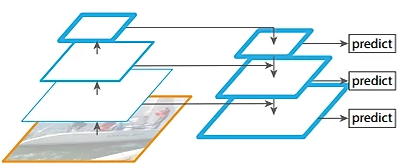
\includegraphics[width=0.5\textwidth]{Figures/fpn.png}
  \caption{Feature Pyramid Network structure~\cite{zhao:obj_survey}.}
  \label{fig:fpn}
\end{figure}

The logistic activation is used to constrain the center coordinates of the box to fall in the range of the grid cell (i.e., between 0 and 1). The objectness score is predicted using logistic regression (1 means perfect overlapping between predicted and ground truth boxes while 0 means no overlapping). For the class predictions, independent logic classifiers are also used. The application of the logistic activation in the predictions of each bounding box, excluding the width and height parameters, is performed by the \textbf{yolo layers}. This new layer added by the YOLOv3 network is used as the ending layer for each scale.

\begin{figure}[!htb]
  \centering
  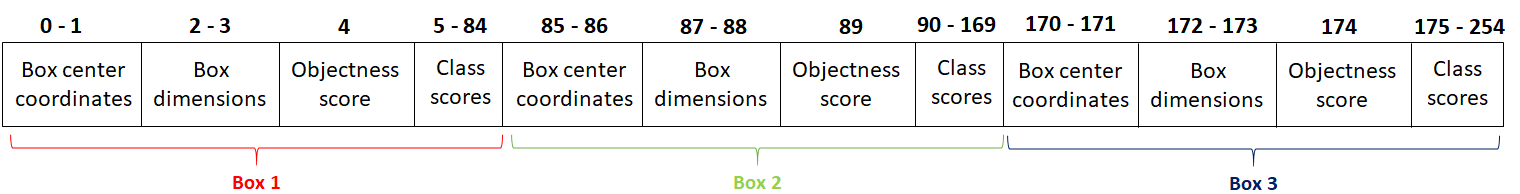
\includegraphics[width=\textwidth]{Figures/grid_cell.png}
  \caption{Constitution of each grid cell.}
  \label{fig:grid_cell}
\end{figure}
\vspace{-0.3cm}

\subsection{Detections phase}

After executing the YOLOv3 network block (Fig.~\ref{fig:yolov3}), there are several candidate bounding boxes for each scale, however, only a few of them correspond to true detections (depending on the number of objects in the image). The true detections correspond to the bounding boxes whose product between the objectness score and the conditional probability of each class is above a given threshold (the default value is 0.5). The bounding boxes can be multilabeled, i.e., can have more than one class. 

Due to detecting objects with three different scales and with three bounding boxes per grid cell, multiple bounding boxes of the same object might be found. The non-maximum suppression is used to remove these multiple detections and consists in the following algorithm~\cite{Redmon2015YouOL}:
\vspace{0.3cm}

\begin{algorithm}[H]
\setstretch{1}
 1) Select bounding box with the highest confidence score \\
 2) Calculate the IoU between selected box and all the remaining boxes \\
 3) Discard boxes whose IoU is greater than a certain threshold (default value is 0.45)\\
 4) Repeat steps 2-4 for the next highest score box until processing all remaining boxes
 \caption{Non-maximum suppresion}
\end{algorithm}

 
\subsection{YOLOv3-Tiny network}

The YOLOv3 network comprises a total of nearly 62 million parameters. The author of this detector~\cite{Redmon2018YOLOv3AI} proposed an alternative network for constrained environments called YOLOv3-Tiny which in turn has a total of approximately 8.8 million parameters. This smaller model presents a mAP (for one IoU of 0.5) of 33.1\% in the COCO dataset and runs at a frame rate of 220 fps in the Titan X GPU. Thus, this version is faster but also less accurate than any other detector in Table~\ref{tab:obj_det_comp}. In the scope of this work, this network can be used as a starting point for acceleration before moving to the YOLOv3 network. 

As represented in Fig.~\ref{fig:yolov3_tiny_ntw}, the YOLOv3-Tiny is composed by 13 convolutional layers, 6 maxpool layers, 2 route layers, 2 yolo layers and 1 upsample layer. In comparison with YOLOv3, this network uses maxpooling instead of convolutions with stride 2 to downsample the feature maps. Besides that, objects are detected with only 2 scales (26x26 and 13x13). No shortcut layers are used.  

\begin{figure}[!htb]
  \centering
  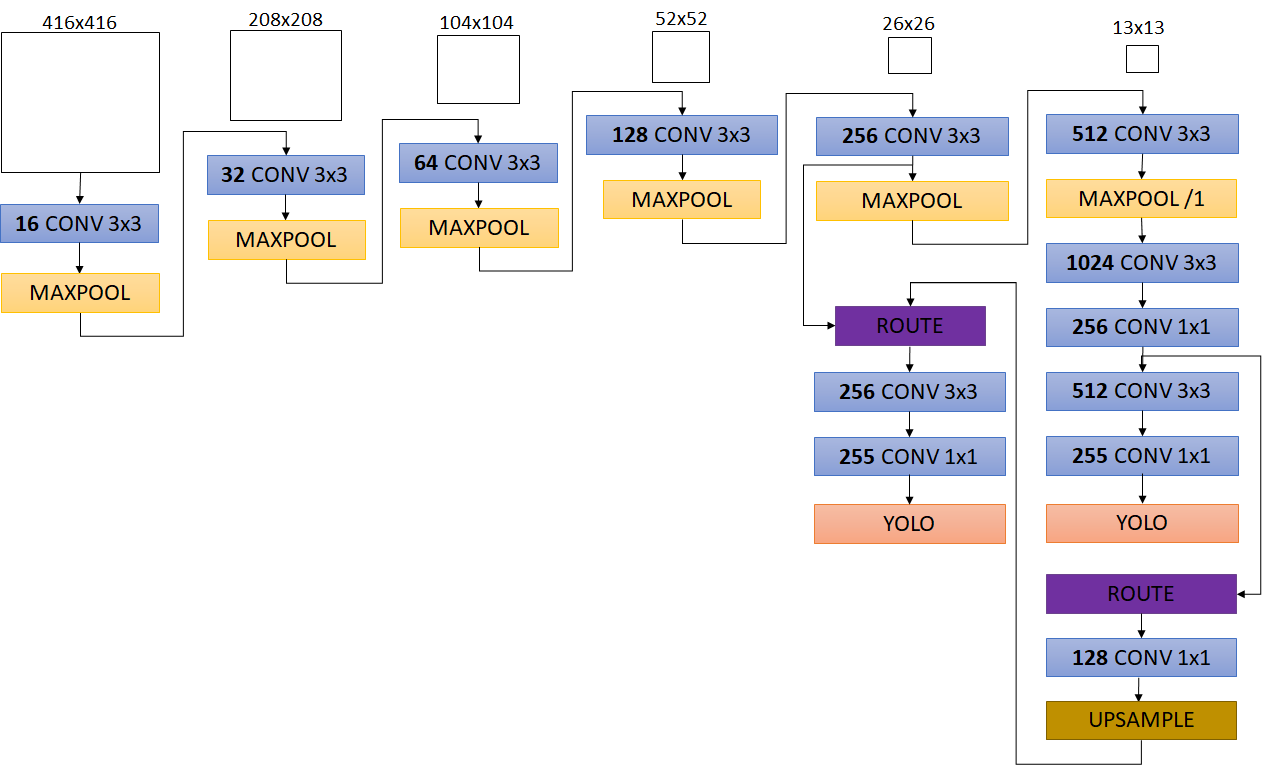
\includegraphics[width=0.85\textwidth]{Figures/tiny.png}
  \caption{YOLOv3-Tiny Network.}
  \label{fig:yolov3_tiny_ntw}
\end{figure}

\subsubsection{Final remarks}

The backbone for feature extraction of the state-of-art object detectors are based on the popular CNNs introduced in the previous chapter. PASCAL VOC and COCO are the most common benchmarks for the evaluation of object detectors where YOLOv3 presents the best trade-off between accuracy and execution time. For this work, the lighter YOLOv3-Tiny network will be initially accelerated using the architecture introduced in the next chapter.   
